% !TeX root = ../main.tex

\chapter{需求分析}
本章将会对课题要实现的分布式对象存储系统进行需求分析。首先会分析本系统的主要使用用户的特点,根据用户的特点和前面章节的介绍,可以得出系统的设计目标,然后分析系统的功能性需求和非功能性需求。

\section{目标用户分析}
在对系统进行详细的需求分析之前,需要对系统的目标用户进行分析,明确这个系统将会为哪些用户服务,这一步对于存储服务来说至关重要,因为对于不同的用户,它们的需求可能是不同的,在为不同的用户提供服务时,需要注意的地方也不一样。

对于存储服务而言,目标用户的分类主要有两个维度,一是使用规模,二是使用方式。下面将会从这两个维度出发,分析系统需要注意的相关事项。

使用规模指的是用户将会向系统存储多少数据,从这个角度分析,可以将用户分为个人用户和企业用户。对于个人用户来说,他们只需要向系统中存储少量的数据来实现自己的业务,如为自己搭建的网站提供非结构化数据的存储服务或者归档大批量冷数据,这些数据的数据量也许对于个人来说是相对庞大的,难以通过个人的硬件来存储它们,但是对于大型的分布式存储系统而言,这些数据的数据量并不算大,大多是TB级别的数据,处理起来相对容易。而对于企业用户,它们要存储的数据量和个人用户相比要大得多,PB级的数据量不在少数,大数据量的存储会对系统提出更高的要求,同时还需要时刻注意这些数据是否需要进行大批量操作,例如用户需要对数据进行迁移时,需要为它们提供一定的支持,确保数据安全以及迁移的高效;在用户连续地向系统中添加数据时,要时刻注意系统的容量是否满足要求,在适当的时候主动进行扩容,保证添加数据不会对其他业务产生影响。

使用方式指的是公有部署还是私有部署。公有部署可以理解为只是将数据存在了云端,用户无需考虑系统的物理设施部署,只使用存储系统提供的服务,这样由云服务提供商提供和管理的服务也被称为公有云。与之相反的则是私有部署,也称为私有云,它是由企业或组织自行搭建的云存储平台,这种平台一般选择将存储系统部署在自己内部的数据中心中,由自己提供相关的物理设施,或者由专门的服务提供商进行托管,这样做的好处是可以自由的选择机器的硬件和软件配置,具有完全的控制权和管理权。一般而言,使用私有部署的一般是大型的企业或组织,它们对存储系统有更高的安全性的要求,它们希望数据能够保存在自己的数据中心中,数据完全由企业或组织进行控制和管理,确保数据的安全,同时它们也希望能够对系统进行定制和管理,根据自己的业务来选择系统的配置,更好地完成存储目标。在为私有部署的用户提供服务时,需要和用户进行充分的沟通,了解用户的需求后,需要指导用户选择合适的物理介质并为系统提供正确的配置,保证系统能够满足用户的需求。

\section{设计目标}
根据以上的分析可知,如果想要为用户更好地解决问题,系统应该实现以下两个设计目标。

1. 低成本

当企业级用户使用分布式对象存储系统时,它们通常需要在系统内保存大量的数据来为上层业务提供服务,不管是在本地进行部署还是以云的方式远程部署,在海量数据面前,都需要考虑存储的成本,尤其是云服务提供者,降低存储的成本可以增加自己的利润。系统除了要完整保存一份文件之外,还需要冗余存储一些额外的数据来为对象数据提供可靠性。系统中可以优化的存储成本主要来源于对象数据的冗余,系统需要给出合理的方案,在提供一定可靠性的前提下,减少冗余数据,降低存储成本。

2. 适合大量小文件存储

在第一章中我们知道,系统主要负责存储非结构化数据,这些数据是由新兴互联网业务而产生的音乐、视频、图片等数据,它们大多都是小文件,而且这些小文件读取较为频繁,因此我们的系统需要格外关注小文件的存储性能。由于操作系统对小文件的IO不友好,所以我们的系统需要提供一定的方案优化小文件的读写性能。

\section{功能性需求}%3.5

本小节进行功能性需求分析,功能性需求分析主要用来列出系统应该具有的功能和服务,通过这部分的分析我们可以将各个功能进行一定的归类,将具有相同操作对象的需求归为一类有助于后续模块的划分,理清它们之间的协作关系。系统的总体用例图如图3.1所示,从系统的总体用例图可以看出系统需要提供四类功能,包括用户数据管理功能、桶数据管理功能、文件管理功能和文件交互功能,接下来将对每类需求进行详细分析。

\begin{figure}[h]
    \centering
    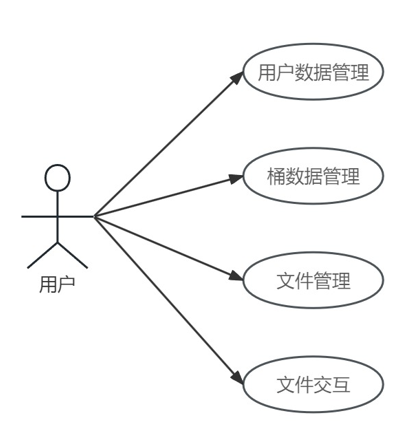
\includegraphics[width=0.48\textwidth]{整体用例图.png}
    \caption{系统总体用例图}
\end{figure}

\subsection{用户数据管理}
本系统会在处理请求时进行鉴权操作,系统的鉴权依赖用户信息,因此若想使用本系统,用户必须先在系统中登记自己的信息。用户数据管理的用例图如图3.2所示,下面将详细介绍系统与用户数据管理相关的功能性需求。

\begin{figure}[h]
    \centering
    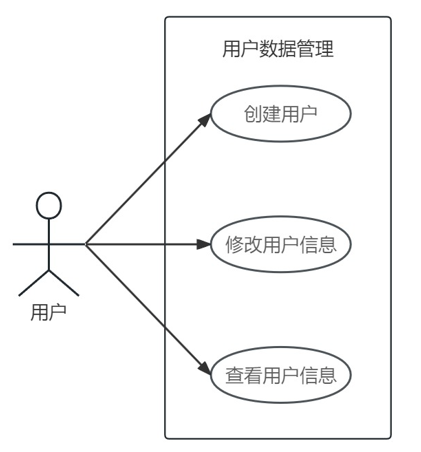
\includegraphics[width=0.5\textwidth]{用户数据管理用例图.png}
    \caption{用户数据管理用例图}
\end{figure}

1. 创建用户

用户第一次使用系统时需要使用创建用户功能来确定访问本系统的用户名和密码,系统提供的其他任何功能都需要对用户的用户名和密码进行鉴权,因此用户务必保存好自己的用户信息。

2. 修改用户信息

用户在登录状态下可以使用修改用户信息功能来修改自己的登录密码。

3. 查看用户信息

用户可以使用查看用户信息功能来获取自己的信息,用户信息中的uid是用户的唯一标识,它不会随着用户名改变而改变,系统通过uid来进行桶的权限管理,用户在获取自己uid后可以将uid告知桶的创建者来获取桶内文件的上传或下载权限。

\subsection{桶数据管理}
在2.1章节中,我们知道对象存储使用桶来管理系统中的文件,它是系统中存储对象的容器,用户上传的每个对象都必须放置在一个桶中。在分析文件相关的操作前,应该先分析桶的相关需求,因为桶是对象的容器,只有创建了桶才能存储对象。对象存储系统中的桶不设置对象的上限,可以进行无限的扩展,但系统中的桶具有唯一性,即一个桶的名称被某用户创建后,其他用户无法创建名称相同的桶,用户创建时务必谨慎。桶数据管理的用例图如图3.3所示,下面将详细介绍系统与桶数据管理相关的功能性需求。

\begin{figure}[h]
    \centering
    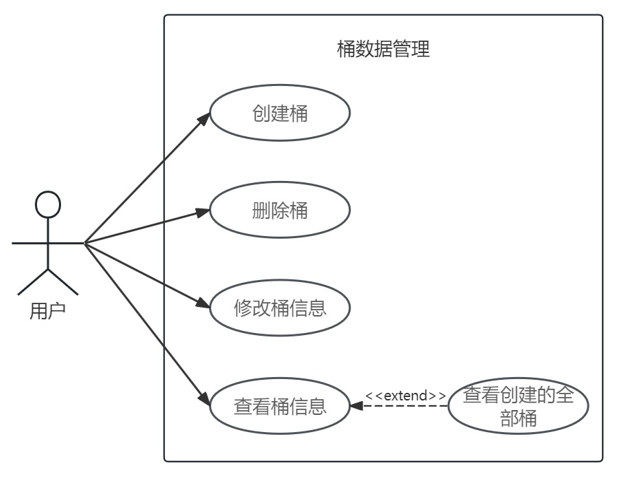
\includegraphics[width=0.7\textwidth]{桶数据管理用例图.png}
    \caption{桶数据管理用例图}
\end{figure}

1. 创建桶

用户若想上传文件,必须要在系统中创建一个桶,在创建桶时需要给出桶的名称,系统应保证这个名称的桶没有被创建过,除此之外,用户在创建桶的时候可以给出这个桶的一些其他信息,比如对桶的访问属性进行控制,指定桶中的对象是公开的还是私有的,若指定为私有则需要用户授权后才能对桶中的对象进行访问。

2. 删除桶

用户可以将指定的桶进行删除,若用户想要删除一个桶,那么这个桶中的文件都将全部删除,用户在进行这个操作时务必谨慎。

3. 修改桶信息

桶在创建之后,桶的名称等信息可以进行修改,其中比较特殊的是桶的访问属性和授权信息。桶的访问属性标记着这个桶内的文件是公有的还是私有的,任何用户都可以下载公有文件,而私有文件只有得到授权的用户才可以下载。授权信息有两个,一个是上传权限的uid组,另一个是下载权限的uid组,在上传权限的uid组中的用户可以向这个桶中上传文件,在下载权限的uid组中的用户可以访问桶内的私有文件。

4. 查看桶信息

这个操作为用户提供查看桶的信息的功能,系统会将桶的信息返回给用户,用户可以通过这个操作得知桶中有多少文件,这个桶总共占据了多少空间,桶的权限配置信息等。除了可以查看单个桶的信息,系统还为用户提供了查看自己创建的全部桶的功能,这个功能是非常实用的,用户可以根据这些信息来对自己的桶进行管理。

\subsection{文件管理}
用户可以对保存在系统中的文件进行管理,文件管理的用例图如图3.4所示,下面将详细介绍系统与文件管理相关的功能性需求。

\begin{figure}[h]
    \centering
    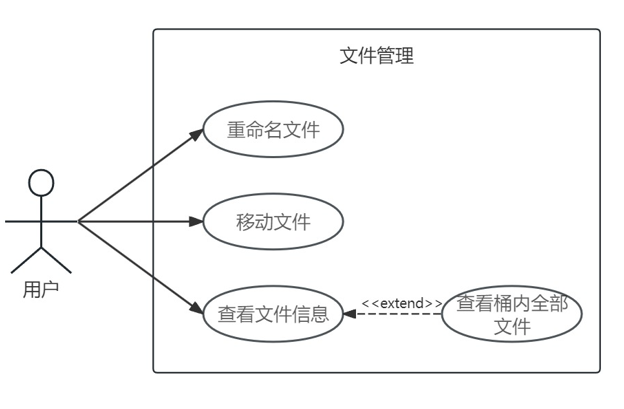
\includegraphics[width=0.7\textwidth]{文件管理用例图.png}
    \caption{文件管理用例图}
\end{figure}

1. 重命名文件

文件的创建者可以将保存在系统内的文件的文件名进行修改,修改过后此文件被用户下载后将显示新的文件名。

2. 移动文件

文件的创建者可以将保存在系统内的文件进行移动,移动之后的文件所属的桶将会改变,同时这个文件的访问权限也会随着它所属的桶发生改变。

3. 查看文件信息

这个操作为用户提供查看文件的信息的功能,需要注意的是,这项功能不是查看文件的具体内容,而是查看文件的相关元信息。系统会将文件的信息返回给用户,用户可以通过这个操作得知文件大小和文件名等相关信息。除了可以查看单个文件的信息,系统还为用户提供了查看某个桶下全部文件信息的功能,用户可以通过这个功能清晰地知道这个桶下保存的文件信息,便于用户管理桶内的文件。

\subsection{文件交互}
用户可以通过接口上传、下载或删除文件,这是本系统的核心功能。需要注意的是,对象存储不支持部分修改或追加,如果需要对对象的内容做出修改,必须重新上传整个对象的数据,将原来的版本进行完全地覆盖,因此对象存储系统适合读多写少的应用,非常适合图片视频等很少需要改动的非结构化的数据。文件交互的用例图如图3.5所示,下面将详细介绍系统与文件交互相关的功能性需求。

\begin{figure}[h]
    \centering
    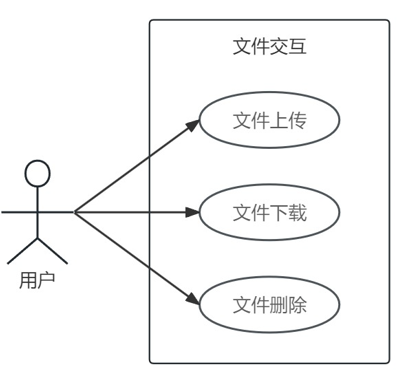
\includegraphics[width=0.5\textwidth]{文件交互用例图.png}
    \caption{文件交互用例图}
\end{figure}

1. 文件上传

文件上传功能将是用户使用频率最高的一项功能,用户可以利用本功能实现文件存储的工作。用户可以向指定的桶中上传文件,系统将会提供接口来接收文件的相关参数和内容,然后将文件的信息存储至元数据服务中,将文件的内容存储至文件存储模块中,整个过程对用户而言是透明的,用户只需调用接口,即可完成文件的上传。

2. 文件下载

文件下载功能可以允许用户从系统中下载文件,这项功能与文件上传功能是本系统的核心功能。和文件上传功能一样,用户需要指定文件的桶和文件名,通过接口向系统获取文件,系统将根据桶和文件名从文件存储模块中获取文件内容,将文件数据发送给用户发起请求的客户端。该功能需保证数据的正确性,在返回给用户之前需要验证文件在存储系统取出后是否和用户上传时一致。

3. 文件删除

文件删除功能是比较容易理解的。文件删除功能允许用户将不需要存储在系统中的文件进行删除,用户需要提供桶名和文件名,通过接口通知系统将文件进行删除。用户可以通过这个功能删除自己上传的文件,将系统中不需要的文件进行删除,释放文件所占据的存储空间。由于此操作十分敏感,因此只允许文件的创建者进行此操作。

\section{非功能性需求}
非功能性需求的分析也是需求分析的重点,因为对非功能性需求的分析能够很好的反映用户对一个对象存储系统的性能需求,它决定了用户是否选择用本系统来进行文件的存储。用户对于系统的非功能性需求有以下几点:

1. 高性能

本系统主要处理海量非结构化数据,这些数据存取的快慢将会直接影响到上层服务的质量,因此用户必然会对存储系统的性能提出一些要求。对于存储系统而言,文件的上传下载速率是最重要的指标,因此在分析性能相关的需求时,我们主要是对文件的上传下载速率提出要求。当前市场上为用户提供服务的存储系统中,在100Mbp/s的网络带宽环境中文件上传速率普遍达到了1MB/s左右,文件的下载速率则在10MB/s左右。用户将希望本系统提供和上述性能相当的存储服务。

2. 可用性

对于许多应用程序而言,在某个时刻无法正确地访问存储的数据意味着巨大的经济损失,因此数据存储的高可用性是一个重要的需求。这要求程序所依赖的存储系统必须保证高度的可用性,用户会期待数据所在的存储系统提供不间断的服务,单台机器发生故障的时候不能影响整个系统的正常运行,无需等待异常节点恢复或者将服务迁移到其他正常节点,同时扩缩容相关的操作也不可以影响业务的运行。

3. 可扩展性

相较于传统的单机存储系统,分布式存储系统能更好地应对存储数据的膨胀,当需要存储的数据逐渐变多的时候,用户会期待存储系统能够进行扩容,且希望扩容过程简单方便,不对原有数据和服务造成影响。

此项要求系统能够为用户提供无容量上限的存储服务,且在物理上对系统扩容时不会影响到用户的正常使用。

4. 安全性

用户可能会将一些不希望公开的信息上传至存储系统中,用户需要存储系统对这些信息进行保护,只有得到文件所有者授权的人才能够访问这些文件。用户会希望数据在存储过程和通信过程中都是安全的,即只允许指定的用户获取文件的内容。

对安全性的需求要求系统能够为文件的存取增加一定的权限限制,用户可以对权限进行管理,通过对权限的操作规定哪些文件可以被所有人访问,哪些文件只能被自己访问。系统需要对数据的访问操作进行相关的鉴权,只有鉴权通过才能够访问系统中的数据。

\section{本章小结}%3.7
本章最开始分析了系统的目标用户,阐述不同用户使用和部署系统的方式是不同的。基于目标用户的分析和前面章节中的内容,得出了系统需要实现低成本和适合大量小文件存储的目标。同时,本章对系统进行了功能性需求和非功能性需求的分析。对于功能性需求,描述了系统应该为用户提供用户数据管理、桶数据管理、文件管理和文件交互的功能,对于非功能性需求,根据本系统的实际应用情况得出了性能、可用性、可扩展性和安全性上的非功能性需求。 
